\documentclass[conference]{IEEEtran}
\usepackage{cite}
\usepackage{amsmath,amssymb,amsfonts}
\usepackage{mathtools}
\usepackage{algorithmic}
\usepackage{graphicx}
\usepackage{textcomp}
\usepackage{xcolor}
\usepackage{hyperref}
\def\BibTeX{{\rm B\kern-.05em{\sc i\kern-.025em b}\kern-.08em
    T\kern-.1667em\lower.7ex\hbox{E}\kern-.125emX}}

% Graphics path
\graphicspath{{./img/}}

% Count figures with sections
\counterwithin{figure}{section}

\begin{document}

% ===== Title ==================================================================

\title{Problem-Oriented Analysis of Self-Organizing Neural Networks}

% ===== Authors ================================================================

\author{\IEEEauthorblockN{Vins Sharma}
    \IEEEauthorblockA{\textit{Electrical and Computer Engineering} \\
        \textit{Carnegie Mellon University} \\
        \texttt{vmsharma@andrew.cmu.edu}
    }
    \and
    \IEEEauthorblockN{Anand Raju}
    \IEEEauthorblockA{\textit{Electrical and Computer Engineering} \\
        \textit{Carnegie Mellon University} \\
        \texttt{amraju@andrew.cmu.edu}
    }
}

\maketitle

% ===== Sections ===============================================================

\begin{abstract}
    Liquid state machines (LSMs) are machine learning models that create more
    biologically plausible neural networks by self-organizing neurons into a
    'liquid'. As such, we aim to analyze a variety of 'liquids' generated off
    unique problems and datasets in order to determine correlations and patterns
    that exist in these graphs. We accomplish this by: (1) Implementing a
    framework to generate LSMs on many problems, and (2) Analyzing generated
    LSMs for overlapping patterns and similarities.
\end{abstract}

\begin{IEEEkeywords}
    liquid state machines, temporal neural networks, random graph models,
    reservoir computing
\end{IEEEkeywords}
\section{Introduction} \label{sec:Introduction}

\subsection{Motivation}

The portion of the brain primarily responsible for human thought and cognitive
function is thought to be the neocortex, which covers the outside shell. The
unfolded neocortex is the size of a dinner napkin, and is made up of tiny
perpendicular 'micro-fibers' called cortical columns \cite{Mountcastle}.

Cortical columns are thought to be the microcircuit that implements all
cognitive thought. Though it is well documented that different regions of the
brain are responsible for different functions, it has been shown \cite{Hawkins}
that the makeup of the cortical column is nearly identical across the entire
neocortex, excluding the inputs. This indicates that a circuit exists that can
be plugged into different problems and solve all of them without significant
modification or significant power consumption.

One approach to designing such a 'perfect' circuit is through induction. In
section \ref{sec:PreviousWork}, we'll discuss this approach in more detail, and
why we are not choosing it. However, another approach is from a top down - We
hope to generate networks from a variety of configurations, look at these
networks, and attempt to understand what similarities exist between them or how
different parameters and problem-specific features affect their design.

\subsection{General Approach}

We start by generating a framework to quickly and easily 'plug in' different
configurations and generate networks. These networks can organize themselves
based on features of the data, and we can analyze how they organize themselves
over time simulations.

With this framework we analyze a variety of unique input configurations to
understand how the network constructs itself. Neurons within the liquid may
reconfigure as they so choose, based closely on their learning algorithm. We
hope to derive some insight into how the network rearranges itself based on the
input data. These similarities and conclusions may serve as the first steps in
constructing a cortical column-like neural circuit.

\subsection{Potential Impacts}

While we do not think we can architect such a circuit as exists in the human
brain, we hope to gain some significant insight into how such a circuit might be
formed based on neuronal dynamics and connectivity.

Several studies have previously looked at brain connectivity from a graph
theoretical viewpoint \cite{Structure-Functional} and have made only passing
comments about the evolution of brain circuitry to handle particular problems.
It has been posited that the brain forms itself to decrease axonal connection
cost from a structural standpoint. However, we choose to look closely at the
functional side of neural circuit development throughout this project. We hope
to demonstrate (in particular) patterns generated from functional connectivity
and analyze how they may be related to the problem being solved.
\section{Previous Work} \label{sec:PreviousWork}

In this section we examine inspirations for our approach, and potential choices.

\subsection{Smith (2023)}

As discussed in \ref{sec:Introduction}, the goal of this project is to get
closer to a cortical column-like neural circuit. Professor Smith's rendition of
his macrocolumn in \cite{Macrocolumn} is an example of the ground-up approach to
solving this problem. He proposes a circuit specialized towards one task -
Having a mouse navigate a maze. Future work in this project involves applying
a slightly modified circuit to another problem.

One major issue with this avenue of thought is the exponentially increasing
amount of effort. In future work, when introducing a new problem, Professor
Smith now has to modify the circuit to solve the new problem while still
preserving the old functionality. As such, we aim to avoid this approach, and
instead take a top-down approach to generalize further.

\subsection{Nair, Shen, Smith (2021)}

This paper \cite{TNN} describes the temporal neuron and a strategy for training
it in an unsupervised way. The temporal neuron simply encodes data inputs on
spike timing lines (in a process known as rate coding). This allows it to
consume significantly less power (as the spike is only on instantaneously), and
also allows for a non-statistical simple unsupervised approach.

For our approach, we implement these temporal neurons, but use them without the
paper's described 'columnar' structure (for the most part). As such, our usage
of temporal neurons is novelly applied in a more arbitrary network structure.

\subsection{Purdy (2016)}

Purdy's paper \cite{Encoding} discusses the best-practices for encoding data in
temporal systems, such as we will throughout this project. He focuses on the
generation of proper sparse distributed representation (SDR) matrices as
good-for-encoding inputs. We apply this knowledge to adapt datasets to temporal
input.

\subsection{Maass (2011)}

Maass defines the liquid state machine (LSM) \cite{LSM} model for reservoir
computing. The LSM has a reservoir with a series of spiking neurons that form
some arbitrary excitation pattern; A separate set of (trained) neurons then read
out this pattern and correlate it to an output. The internals of the reservoir
can be structured in any way, but are conceptually similar to self-organizing
maps \cite{Kohonen}.

Kohonen posits, through his work, that arbitrary higher dimensional features of
a problem are encoded into the graph's organization for a self-organizing map.
As such, we analyze the organization of the reservoirs in order to draw
possible conclusions about the features of the problem.

\subsection{Hazan, Manevitz (2012)}

Hazan and Manevitz \cite{LSM Constraints} propose in their paper that the LSM
previously defined by Maass is not a good model due to its network's robustness,
and that a more robust model would better represent the brain. They draw a new
conclusion towards small-world assumptions in graph topology being key to
solving this problem. We re-test this hypothesis in our work.
\section{Approach} \label{sec:Approach}

\subsection{Datasets}

Throughout our project, we apply a few datasets and analyze their generated
graphs. The datasets we use are, relatively speaking, orthogonal to each other -
They solve fundamentally different problems. As such, any similarities may be in
response to parameter changes, the network structure, or 'problem-solving'
itself.

Our first benchmark is the MNIST dataset \cite{MNIST Dataset}. This dataset
requires the tools of image recognition and classification, and is popular in
machine learning projects.

From there, we look at the Numenta Anomaly Benchmark dataset \cite{NAB Dataset}.
Anomaly detection is a problem that temporal neural networks generally
specialize in, so we analyze these as well.

Finally, we generate and analyze a network for the NFL Big Data Bowl dataset
\cite{NFL Dataset}. This network would perform prediction for the next 'play'
(e.g. pass or rush) based on the previous play's characteristics.

\subsection{Network Configuration}

Before discussing our network, we introduce our system. We define a temporal
liquid state machine (TLSM) as an input vector, encoded in time-based spikes,
followed by a reservoir of temporal neurons, and finally a singular output
column (with winner-takes-all lateral inhibition). The input vector uses
encoding strategies discussed in \cite{Encoding}, and the output column is
identical to the one described in \cite{TNN}.

\begin{figure}[h]
    \centering
    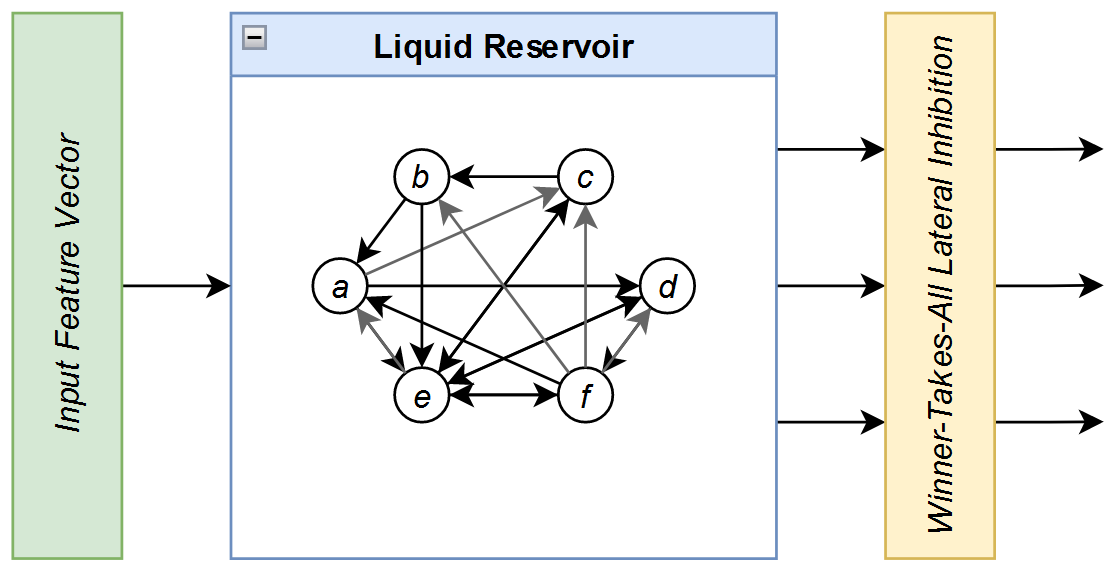
\includegraphics[scale=0.25]{tlsm_diagram.png}
    \caption{Diagram of a temporal liquid state machine (TLSM).}
    \label{fig:tlsm_diagram}
\end{figure}

The reservoir is the focus of network analysis, containing a series of neurons.
This graph of neurons will change over time with training and with STDP rules,
adding and removing connections arbitrarily in response to the inputs. The
neuron activation function is also a hyperparameter of the network.

Furthermore, a 'seed' configuration for the network may be specified, indicating
its initial connectivity. This seed configuration is generated through a
number of random graph algorithms, and is a hyperparameter of the network.

\subsection{Assumptions}

While we vary a variety of parameters (such as neuron activation function), we
assume that the underlying temporal neurons function as a strong analogue for
biological processes. This assumption allows us to generalize our results to
neural basis of cognition rather than design of artificial neural networks.

\subsection{Analysis}

The focus of analysis is the network generated within the liquid reservoir. This
liquid has nodes of neurons and edges of weighted synapses.

We test the robustness claim of \cite{LSM Constraints} by analyzing the
connectivity of these networks over their growth. We also analyze diameter in
order to understand the 'distance' between neurons in the network (and the
amount of time it takes for a spike to propagate).

\subsection{Research Questions}

Through these network features, and more, we aim to understand the following:

\begin{enumerate}
    \item Why did the network configure itself the way it did?
    \item How do networks of different problems compare to each other?
\end{enumerate}
\section{Network Configuration} \label{sec:Network Configuration}

We introduce our system. We define a temporalliquid state machine (TLSM) as an
input vector, encoded in time-based spikes, followed by a reservoir of temporal
neurons, and finally a singular output column (with winner-takes-all lateral
inhibition). The input vector uses encoding strategies discussed in
\cite{Encoding}, and the output column is identical to the one described in
\cite{TNN}.

\begin{figure}[h]
    \centering
    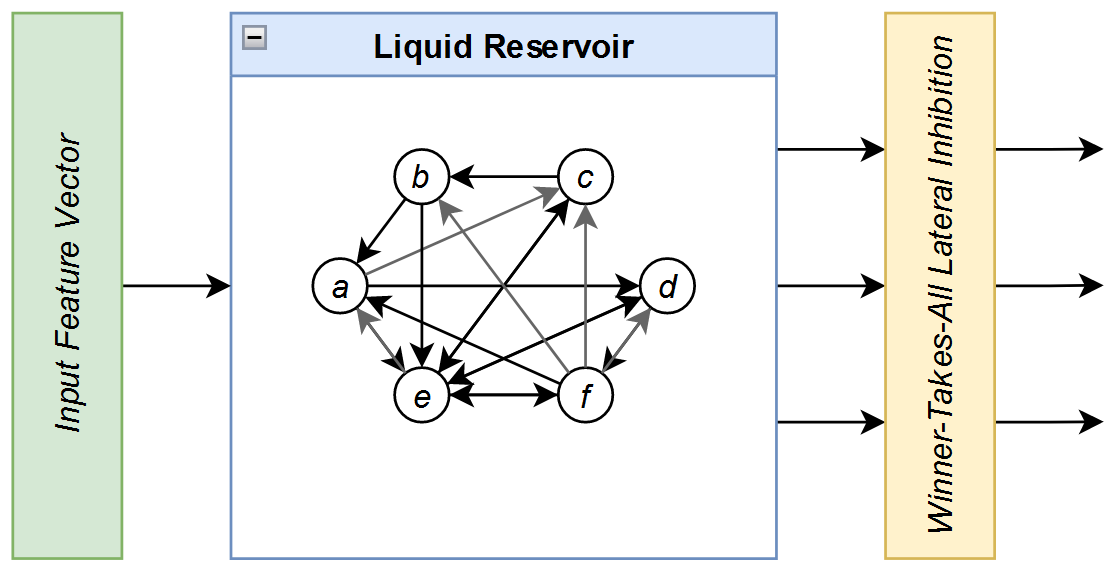
\includegraphics[scale=0.25]{tlsm_diagram.png}
    \caption{Diagram of a temporal liquid state machine (TLSM).}
    \label{fig:tlsm_diagram}
\end{figure}

\subsection{Input Encoding}

The input vector is a series of time-encoded one-hot vector spikes. For the
example of MNIST data, the input $28 \times 28$ image is flattened into a
$784 \times 1$ vector. Each element of the vector is subsequently expanded into
a $t_{res} \times 1$ one-hot time-spike encoding vector, where the time
represents the pixel's brightness. If the pixel is simply black, the time is
set to infinity; Any low values will round to zero. More input processing may
be necessary for particular problems - In order to ensure that bright pixels do
not 'dominate' the input, the image may be duplicated and inverted to include a
pos-neg encoding scheme.

The temporal resolution, $t_{res}$, is an important hyperparameter of this
encoding scheme, as with higher resolutions the network may take longer to train
and infer. However, as resolution increases, so too does accuracy.

\subsection{Temporal Neuron}

The temporal neuron is a simple model of a neuron that fires in response to a
series of time-spiking encoded inputs. It is mainly discussed in \cite{TNN}, but
we will briefly summarize its functionality here. Chiefly, the temporal neuron
consumes significantly less power than point-integrator alternatives, and is
generally trained in an unsupervised fashion. The temporal neuron is also
considered a more biologically plausible neuron model, as it more closely
relates to the Hodgkin-Huxley model \cite{Hodgkin-Huxley} of a neuron.

The temporal neuron takes in a series of inputs on a number of lines, generally
encoded in a one-hot manner. Each line has an internal weight represented with
it, encoding the dendritic segment's channel strength from the pre-synaptic
neuron. The input lines are multiplied and summed, and the result increases the
neuron's body potential. When the body potential reaches a threshold $\theta$,
the neuron will spike, sending a high signal on its axonal output line, and the
body potential will reset.

The method in which neurons accumulate body potential is a hyperparameter of the
network. The simplest implementation strategy is Step No-Leak (SNL) neurons,
where the body potential instantly adds. A more involved strategy is the
Ramp No-Leak (RNL) neuron, where the body potential will increase over time
corresponding to the input. The Leaky Integrate-and-Fire (LIF) neuron is a more
biologically plausible model as well, where the body potential will (in addition
to the ramping nature of the RNL neuron) 'leak' out over time, decreasing the
excitation rate.

\subsection{STDP Training}

We implement Spike-Timing-Dependent Plasticity (STDP) training rules for the
temporal neurons within our work. STDP rules are based closely on Hebbian theory
\cite{STDP}, though the actual definitions of the rules vary. For our
implementation, we utilize unsupervised STDP rules as well as supervised STDP
rules as proposed in \cite{TNN} for some input spike time $t_i$ and output time
$t_j$:

$$
    \Delta w_{ij} = \begin{cases}
        \begin{matrix}
            B(\mu_c)  & \text{ if } t_i\leq t_j, & t_i\neq \infty, & t_j\neq\infty \\
            -B(\mu_b) & \text{ if } t_i > t_j,   &                 & t_j\neq\infty \\
            B(\mu_s)  & \text{ if }              & t_i\neq \infty, & t_j=\infty
        \end{matrix}
    \end{cases}
$$

The parameters of $\mu_c$, $\mu_b$, and $\mu_s$ are the STDP capture, backoff,
and search parameters. They represent finite probabilities, and the notation of
$B(\mu_*)$ refers to the choosing of a Bernoulli random variable. This
implementation of STDP is unsupervised; \cite{TNN} also proposes a supervised
approach to training called R-STDP, which will be used for an output layer.

\subsection{Reservoir}

The reservoir is the focus of network analysis, containing a series of temporal
neurons arranged in a randomly connected graph, or a 'liquid'. This graph of
neurons will change over time with training and with STDP rules, adding and
removing connections arbitrarily in response to the inputs.

Furthermore, a 'seed' configuration for the network may be specified, indicating
its initial connectivity. This seed configuration $W_0$ is generated through a
number of random graph algorithms, and is a hyperparameter of the network.

\subsection{Discriminant Column}

The output discriminating column, responsible for classifying the state of the
liquid, is implemented as a TNN minicolumn as described in \cite{TNN}. The
minicolumn is a series of $n$ neurons (for $n$ output classifications), and is
furthermore fed into a winner-takes-all lateral inhibition (WTA-LI) layer. The
WTA-LI layer implements the biological function of astroglia, inhibiting outputs
of neurons as necessary. STDP rules for this output column also take into
account the output time $t_j$ as the time when the entire column spikes.

With the WTA-LI column, the first neuron to spike inhibits all other neurons,
and will dominate the output. Other forms of inhibition and astrocyte modelling
have been explored in related work (see \cite{Astrocyte}), but will not be
explored within our project.
\section{Experimental Setup and Results} \label{sec:ExperimentalSetup}

Our first benchmark and first goal is the MNIST dataset \cite{MNIST Dataset} and
the creation of a framework that can automate this procedure. In this milestone
we have completed the design for the Step No-Leak (SNL) neuron, as well as the
input vector and liquid reservoir. Other neuron types are in progress, and the
temporal mini-column enabling supervised training has yet to be implemented.

We also have a number of seed networks implemented and ready for initializing
and training weights - These include Erdos-Renyi, Watts-Strogatz, and Barabasi-
Albert random graphs. We also have a fully-connected structure for comparison.
\section{Conclusions} \label{sec:Conclusions}

Our project presents a framework for generating and analyzing self-organizing
neural networks in order to derive insight into the neural basis for cognition
through the orientation of the problem. Through analyzing the networks, we hope
to uncover similarities and understand how these structures may organize and
train to particular problems.

\subsection{Plans for Next Milestone}

By the end of November, we plan to complete our network generation framework,
alongside a number of other seed networks and neuron types. We also plan to
generate and analyze the generated MNIST network \cite{MNIST Dataset} as well
as the NFL big data bowl network \cite{NFL Dataset}.

\subsection{Contribution}

For this milestone, Vins focused on the input vector and SNL neuron
implementation. In contrast, Anand focused on the initial graph organization and
seed matrix generation. Both teammates contributed to the overall design of the
TLSM generator framework, and both teammates will contribute to design and
analysis of the MNIST network \cite{MNIST Dataset}.

In the future, Anand will be responsible for the design and analysis of an NFL
data network \cite{NFL Dataset}, and Vins will be responsible for the NAB
network \cite{NAB Dataset}.
\begin{thebibliography}{00}

    \bibitem{TNN}
    H. Nair, J. P. Shen, and J. E. Smith.
    ``A Microarchitecture Implementation Framework for Online Learning with Temporal Neural Networks.''
    \textit{IEEE Computer Society Annual Symposium on VLSI (ISVLSI)}
    (2021).

    \bibitem{LSM}
    W. Maass.
    ``Liquid State Machines: Motivation, Theory, and Applications.''
    \textit{Computability in Context: Computation and Logic in the Real World}
    (2011).

    \bibitem{LSM Constraints}
    H. Hazan, L. M. Manevitz.
    ``Topological Constraints and Robustness in Liquid State Machines.''
    \textit{Expert Systems with Applications}
    (2012).

\end{thebibliography}

\end{document}
